% Generated by paper/build_parameter_figures.py; do not hand edit.
% Source: CURRENT_RESULTS_TABLES.md; normalized SHA-256 babf158f4e596c41a220fcc2993a466fc538dc0758ddf9f78e6d62741be570e6
% Rounded binary64 diagnostics, not new outward-rounded certificates.
\begin{figure}[tb]
\centering
\begin{minipage}[t]{.485\linewidth}
\centering
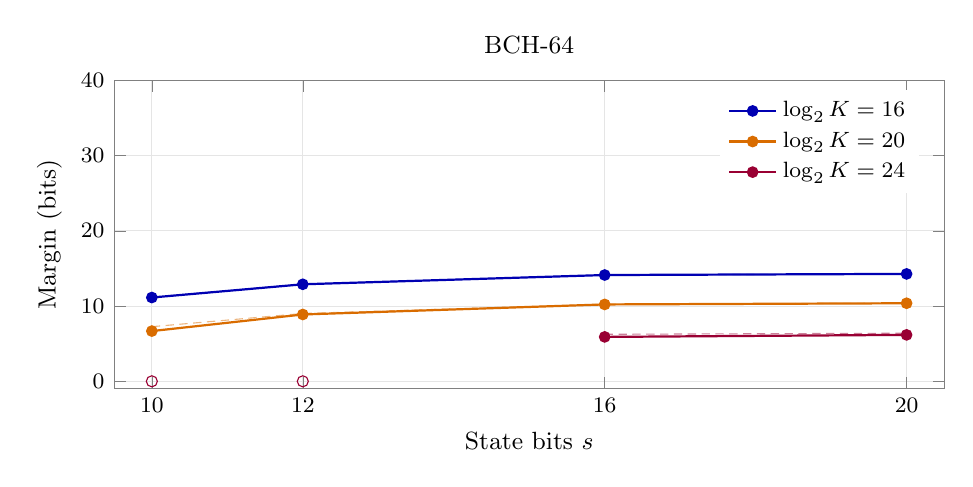
\begin{tikzpicture}
\begin{axis}[tick label style={font=\footnotesize},label style={font=\small},title style={font=\small},grid=major,grid style={black!10},axis line style={black!50},legend style={font=\footnotesize,draw=none},width=\linewidth,height=5.5cm,title={BCH-64},xlabel={State bits $s$},ylabel={Margin (bits)},xmin=9.5,xmax=20.5,ymin=-1,ymax=40,xtick={10,12,16,20},ytick={0,10,20,30,40},legend pos=north east,]
\addplot[blue!70!black,thick,mark=*,mark size=1.7pt,unbounded coords=jump] coordinates {(10,11.134982000) (12,12.891468000) (16,14.123995000) (20,14.271217000)};
\addplot[blue!70!black,densely dashed,opacity=.5,unbounded coords=jump,forget plot] coordinates {(10,11.180859200) (12,12.901190020) (16,14.125694260) (20,14.272276680)};
\addlegendentry{$\log_2 K=16$}
\addplot[orange!85!black,thick,mark=*,mark size=1.7pt,unbounded coords=jump] coordinates {(10,6.674265000) (12,8.880604000) (16,10.215546000) (20,10.371924000)};
\addplot[orange!85!black,densely dashed,opacity=.5,unbounded coords=jump,forget plot] coordinates {(10,7.258641000) (12,9.013821000) (16,10.239631800) (20,10.386947400)};
\addlegendentry{$\log_2 K=20$}
\addplot[purple!80!black,thick,mark=*,mark size=1.7pt,unbounded coords=jump] coordinates {(10,nan) (12,nan) (16,5.901222000) (20,6.171264000)};
\addplot[purple!80!black,densely dashed,opacity=.5,unbounded coords=jump,forget plot] coordinates {(10,nan) (12,nan) (16,6.246809000) (20,6.394199000)};
\addlegendentry{$\log_2 K=24$}
\addplot[only marks,purple!80!black,mark=o,mark size=2pt,forget plot] coordinates {(10,0.000000000) (12,0.000000000)};
\end{axis}
\end{tikzpicture}
\end{minipage}
\hfill
\begin{minipage}[t]{.485\linewidth}
\centering
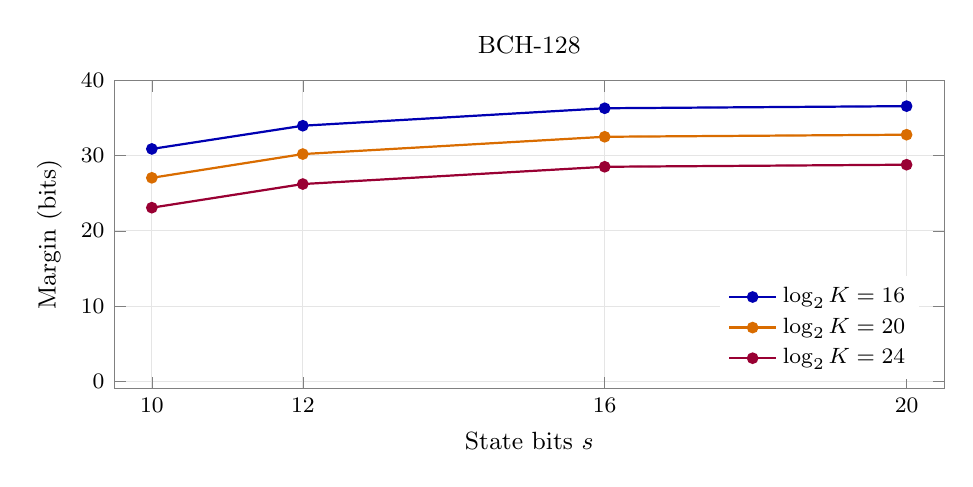
\begin{tikzpicture}
\begin{axis}[tick label style={font=\footnotesize},label style={font=\small},title style={font=\small},grid=major,grid style={black!10},axis line style={black!50},legend style={font=\footnotesize,draw=none},width=\linewidth,height=5.5cm,title={BCH-128},xlabel={State bits $s$},ylabel={Margin (bits)},xmin=9.5,xmax=20.5,ymin=-1,ymax=40,xtick={10,12,16,20},ytick={0,10,20,30,40},legend pos=south east,]
\addplot[blue!70!black,thick,mark=*,mark size=1.7pt,unbounded coords=jump] coordinates {(10,30.878456000) (12,33.963512000) (16,36.285079000) (20,36.564526000)};
\addplot[blue!70!black,densely dashed,opacity=.5,unbounded coords=jump,forget plot] coordinates {(10,30.878456160) (12,33.963512013) (16,36.285079001) (20,36.564526000)};
\addlegendentry{$\log_2 K=16$}
\addplot[orange!85!black,thick,mark=*,mark size=1.7pt,unbounded coords=jump] coordinates {(10,27.041016000) (12,30.197059000) (16,32.494912000) (20,32.769598000)};
\addplot[orange!85!black,densely dashed,opacity=.5,unbounded coords=jump,forget plot] coordinates {(10,27.041018141) (12,30.197059153) (16,32.494912011) (20,32.769598006)};
\addlegendentry{$\log_2 K=20$}
\addplot[purple!80!black,thick,mark=*,mark size=1.7pt,unbounded coords=jump] coordinates {(10,23.073433000) (12,26.213317000) (16,28.508122000) (20,28.782539000)};
\addplot[purple!80!black,densely dashed,opacity=.5,unbounded coords=jump,forget plot] coordinates {(10,23.073466424) (12,26.213319411) (16,28.508122173) (20,28.782539091)};
\addlegendentry{$\log_2 K=24$}
\end{axis}
\end{tikzpicture}
\end{minipage}

\caption{The state curve at three message lengths, with $t=64$ fixed.
Only the four marked states are compared at every length. Solid and faint
dashed curves denote full and $q=1$ margins. Open circles on the baseline
flag negative full-bound margins, rather than zero-margin measurements;
no line crosses these points. Smaller states amplify the higher-occupancy
loss for BCH-64 at the largest message length.}
\label{fig:finite-k-s}
\end{figure}
